\clearpage
\section{Problembeskrivelse}
\label{problemBeskrivelse}

%Her kan du skrive om din problembeskrivelse

I et nevron er det alltid et elektrisk potensiale over en eller annen membran, og når potensialet blir høyt nok, fyres nevronet av og så blir det en påfølgende utladning En modell for utladningen etter avfyring er Fitzhug-Nagumo-likningene som sett i \autoref{eq:fitzhug_nagumo}. Og denne diferensiallikningen kan brukes til å moddelere et EKG signal som vist i \autoref{fig:ekg_simple_1}. I \autoref{fig:ekg_real_1} er et eksempel på et faktisk EKG signal.

\begin{equation}
    \label{eq:fitzhug_nagumo}
    \begin{cases}
        \dot{v} = (v-a)(1-v)v-w \\
        \dot{w} = bc - cw
    \end{cases}
\end{equation}

\begin{figure}[!h]
    \centering
    \begin{minipage}[c]{0.4\textwidth}
        \centering
        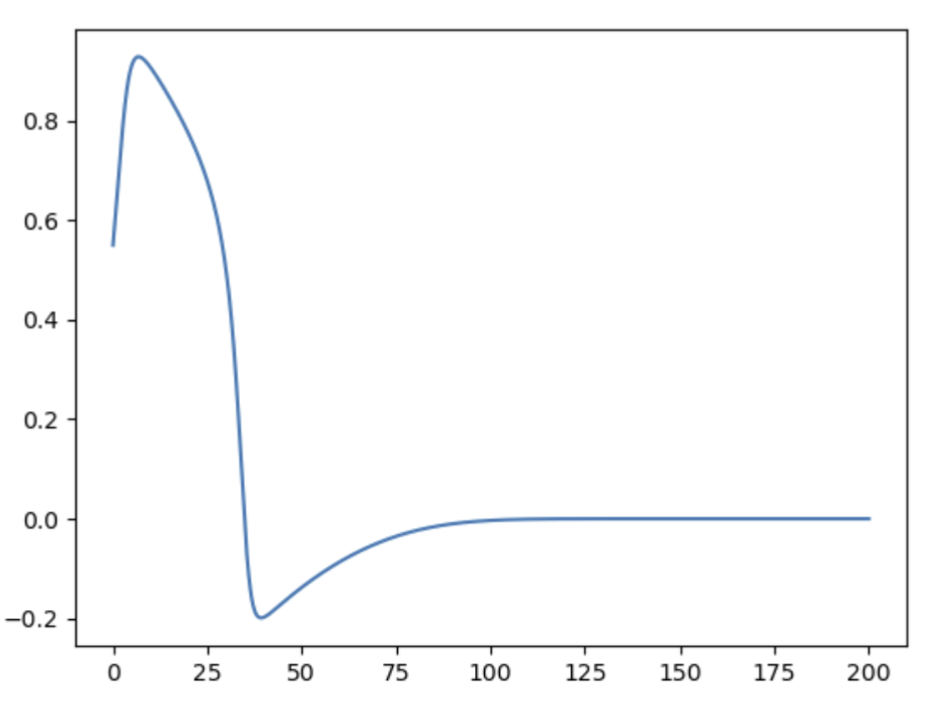
\includegraphics[width=1.1\textwidth]{./Bilder/Enkel_EKG_v0.png} 
        \caption{EKG gitt den matetamtiske funksjonen \newline $\dot{v} = (v-a)(1-v)v-w$ \newline $\dot{w} = bc - cw$.}
        \label{fig:ekg_simple_1}
    \end{minipage}
    \hfill
    \begin{minipage}[c]{0.5\textwidth}
        \centering
        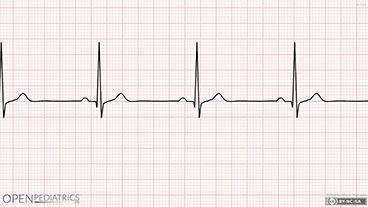
\includegraphics[width=1.1\textwidth]{./Bilder/ECG1920x1080.jpg} 
        \caption{Et faktisk EKG signal.}
        \label{fig:ekg_real_1}
    \end{minipage}
\end{figure}

Denne oppgaven vil hovedsakelig fokusere på tre forskjellige punkter:

\newcounter{boxlblcounter}  
\newcommand{\makeboxlabel}[1]{\fbox{#1.}\hfill}% \hfill fills the label box
\newenvironment{boxlabel}
  {\begin{list}
    {\arabic{boxlblcounter}}
    {\usecounter{boxlblcounter}
     \setlength{\labelwidth}{3em}
     \setlength{\labelsep}{0em}
     \setlength{\itemsep}{2pt}
     \setlength{\leftmargin}{1.5cm}
     \setlength{\rightmargin}{2cm}
     \setlength{\itemindent}{0em} 
     \let\makelabel=\makeboxlabel
    }
  }
{\end{list}}


\begin{boxlabel}
\item Hovedfokuset til denne oppgaven blir å finne vårt egnet EKG signal for deretter å finne en modell som kan beskrive dette signalet, med faktiske verdier for parametrene i modellen. 
\item Finne en bedre mattematisk modell for EKG signalet, enten på nettet eller ved egen forskning.
\item Lage en prototype EKG krets som kan brukes til å måle vårt eget EKG signal, og sammeligne vår data med data fra en EKG måling fra profesjonellt utstyr.
\end{boxlabel}